\documentclass[conference]{IEEEtran}

\usepackage[english]{babel}
\usepackage{blindtext}
\usepackage{xcolor}

\usepackage[nomain, toc, acronym]{glossaries}
\usepackage{subfig}
\usepackage{booktabs}
\usepackage{hyperref}
\usepackage{amsmath}
\usepackage{amssymb}
\usepackage{graphicx}
\usepackage{booktabs}
\usepackage{multirow}

\newacronym{dl}{DL}{Deep Learning}
\newacronym{rl}{RL}{Reinforcement Learning}
\newacronym{ours}{OurSolution}{OurSolution}
\newacronym{cca}{CCA}{Congestion Control Algorithms}
\newacronym{aqm}{AQM}{Active Queue Management}
\newacronym{rtt}{RTT}{Round Trip Time}
\newacronym{fq}{FQ}{Fair Queuing}
\newacronym{ml}{ML}{Machine Learning}
\newacronym{bdp}{BDP}{Bandwidth Delay Product}
\newacronym{mae}{MAE}{Mean Absolute Error}
\newacronym{mse}{MSE}{Mean Squared Error}
\newacronym{qoe}{QoE}{Quality of Experience}



\newcommand{\mynote}[3]{
    \fbox{\bfseries\sffamily\scriptsize#1}
    {\small$\blacktriangleright$\textsf{\emph{\color{#3}{#2}}}$\blacktriangleleft$}}

\newcommand{\todo}[1]{\mynote{TODO}{#1}{red}}

\begin{document}
\title{Online Learning of Per-flow Queuing Policies using Deep Reinforcement Learning}

\author{\IEEEauthorblockN{Maximilian Bachl, Joachim Fabini, Tanja Zseby}
\IEEEauthorblockA{Technische Universität Wien\\
firstname.lastname@tuwien.ac.at}}

\maketitle

\begin{abstract}
The increasing number of different, incompatible congestion control algorithms has led to an increased deployment of fair queuing. Fair queuing isolates each network flow and gives it a separate queue. It can thus guarantee fairness for each flow even if the flows' congestion controls are not inherently fair. So far, each queue in the fair queuing system either has a fixed, static maximum size or is managed by an Active Queue Management algorithm (AQM) like CoDel. In this paper we design and implement an AQM mechanism that dynamically learns the optimal buffer size for each flow with respect to a specified utility function. We show that our Deep Learning based algorithm can correctly fingerprint each flow and assign the optimal queue size. Besides that we also show that our mechanism can even learn completely on-line and can continuously adapt. Finally we demonstrate that the computational overhead of our approach is sufficiently low to allow for deployment on regular hardware. 
\end{abstract}

\section{Introduction}

New \gls{cca} for TCP and QUIC are still being introduced, with one of the most prominent ones in recent years being BBR \cite{cardwell_bbr:_2016}\todo{Add more refs}. While new \glspl{cca} are commonly being designed with compatibility to other \glspl{cca} in mind, often they do not share the link completely fairly with older \glspl{cca}\todo{Add more refs}. Besides that, network flows using the same \gls{cca} can also be unfair to each other: For example, BBR favors flows with a high \gls{rtt}, while New Reno favors those with a low one \cite{turkovic_interactions_2019,turkovic_fifty_2019}. This unfairness can be mitigated by using \gls{fq} at the bottleneck link, isolating each flow from all other flows and assigning each flow an equal share of bandwidth \cite{dumazet_pkt_sched:_2013}. 

The question of how to manage each queue then arises: The simplest solution is using a static buffer size (queue size) for each flow. Another solution is to use an advanced \gls{aqm} mechanism like CoDel for each flow. CoDel aims to keep the queue length under a certain threshold, making sure that the queuing delay was smaller than 5\,ms in the last 100\,ms at least once. Otherwise it drops packets to decrease the queue length. Both of these approaches do not differentiate between flows: They apply the same logic to each flow no matter its congestion control and no matter the current bandwidth and \gls{rtt}. \cite{bachl_cocoa_2019} showed that this behavior leads to some flows not being able to claim the full bandwidth that they are entitled to. Other flows might achieve the full bandwidth but keep an unnecessary standing queue. \cite{bachl_rax_2019} proposed a mechanism that adjusts the queue of each flow based on its congestion control and showed that it works well for several common \glspl{cca}. However, their algorithm has parameters that have to be manually adjusted and is not guaranteed to work for every \gls{cca} because it makes the assumption that each flow's congestion window follows a zigzag pattern. Furthermore, their approach is only tailored towards flows that always have data to send while the behavior for application limited flows, that also have idle periods, is not clear. 

Instead of a hand-crafted solution like the existing ones, we argue that instead operators of network hardware should be able to simply specify a utility function, and the \gls{aqm} then automatically finds the right queuing policy based on that utility function using \gls{ml}. 

To make our work reproducible and to encourage further research, we make the code, figure and data of this work publicly available\footnote{\url{https://github.com/CN-TU/reinforcement-learning-for-per-flow-buffer-sizing}}. 

\section{Concept}

\begin{figure}[h]
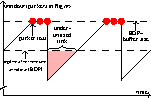
\includegraphics[width=\columnwidth]{figures/cocoa_illustration_too_little.pdf}
\caption{If the buffer is too small, loss-based \glspl{cca} cannot fully utilize the link since they send too few data following the multiplicative decrease that occurs after packet loss.}
\label{fig:tooLittle}
\end{figure}
\begin{figure}[h]
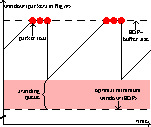
\includegraphics[width=\columnwidth]{figures/cocoa_illustration_too_much.pdf}
\caption{If the buffer is too large, loss-based \glspl{cca} keep an unnecessary standing queue not required for achieving full link utilization.}
\label{fig:tooMuch}
\end{figure}
\begin{figure}[h]
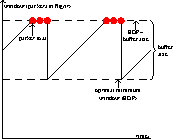
\includegraphics[width=\columnwidth]{figures/cocoa_illustration_perfect.pdf}
\caption{For a flow controlled by New Reno, if the buffer is the same size as the \gls{bdp}, no standing queue exists and the full bandwidth is achieved.}
\label{fig:perfect}
\end{figure}

If the buffer for a flow is too small, this flow cannot achieve the full bandwidth as shown in \autoref{fig:tooLittle}. On the other side, if the buffer is too large (\autoref{fig:tooMuch}), the flow can achieve the full bandwidth but a standing queue exists, which causes unnecessary delay.  

For the popular \gls{cca} \textit{New Reno}, the buffer size that is necessary in a fair queuing setting is one \gls{bdp}, meaning $\textit{speed}\times\textit{delay}$ (\autoref{fig:perfect}). This is because its multiplicative decrease factor is $0.5$, meaning that after packet loss, the congestion window is halved. For other \glspl{cca} like \textit{Cubic} \cite{ha_cubic:_2008}, the multiplicative decrease factor is $0.7$, meaning that the congestion window is reduced to 70\% of its previous value upon packet loss. This means that the minimum buffer size required to achieve full throughput for a Cubic flow is $\left(\frac{1}{0.7}-1\right)\times \textit{BDP}$, which is around 43\% of the \gls{bdp} and thus less than for New Reno. It follows that an adaptive fair \gls{aqm} must learn the underlying \gls{cca} from a flow to adjust the buffer optimally. 

Because optimal buffer size for many \glspl{cca} depends on the \gls{bdp} and thus on the bandwidth and the delay (\gls{rtt}), for example, a flow only having half the \gls{rtt} of another one only needs half its buffer size to achieve full bandwidth. 

To learn an optimal \gls{aqm} policy, we specify a utility function, which the \gls{ml} based \gls{aqm} then should learn. A simple utility function is for example:

\begin{align}
\textit{Utility} = \textit{bandwidth}-\alpha\times\textit{queue size}
\end{align}

In this utility function, the choosable parameter $\alpha$ specifies the tradeoff that is chosen between the bandwidth and the buffer size. With $\alpha$ going to zero, the optimum policy approaches the one in which the buffer size is large enough that a flow never underutilizes the link but at the same time the buffer is never going to be larger than necessary if this doesn't provide a benefit in throughput. 

Our \gls{ml} system uses the above utility function to learn the optimal behavior. \gls{ours} computes features for each flow after every packet it receives and then outputs the optimal buffer size that it deems to maximize the utility function. As the input we use the following features: 
\begin{itemize}
\item queue size
\item standard deviation of the queue size 
\item maximimum allowed buffer size
\item rate of incoming data
\item rate of outgoing data
\item time since the last packet loss
\end{itemize}
We do not use these features directly but instead use 10 exponentially weighted averages of them for each feature with weights of $2^{-4}$, $2^{-5}$, ... , $2^{-13}$. The advantage of using exponentially weighted averages is that they do not occupy any space in memory except for their own values. This is opposed to regular moving averages, which have to keep the entire window of data in memory. 

One difficulty is to get an exponentially moving average for the rate of incoming/outgoing packets because computing the average of rates is mathematically not easily possible: Instead we compute the exponentially moving average of the interarrival times of incoming packets and the interdeparture times of outgoing packets. We then invert this number to get the rate. Another issue here is that numeric instability and division by zero errors can occur using this approach. Thus, we only use the exponential average with a weight of $2^{-n}$ after at least $n$ packets have arrived. Otherwise we set it to zero. 

Using these features gives us a feature vector of $6\times 10 = 60$ features at each point in time. The features are fed into a neural network which has one output: The deemed optimal queue size.  

\section{Implementation} 

We implement \gls{ours} in the network simulator ns-3 \cite{nsnam_ns-3_nodate} and integrate Pytorch's \cite{paszke_pytorch_2019} C++ API into ns-3 for the \gls{dl}. All our code runs on the CPU. 

For the simulations we randomly draw a bandwidth (5 to 25\,Mbit/s), a delay (5 to 25\,ms) and duration (3.75\,ms to 6.25\,ms) and a \gls{cca} (New Reno or BIC \cite{lisong_xu_binary_2004}). We use New Reno because it is one of the oldest, most widely deployed \glspl{cca} and BIC because it is similar to Cubic, which is the default in Linux, Windows and most other OSs currently. We cannot use Cubic itself because there is no stable Cubic implementation in ns-3 currently. As the experiment time (the time at which the experiment is launched to determine if a larger or smaller buffer size would be better), we use a random number between 0 and half of the flow duration of the current flow. 

For the simulation we use two hosts that are directly connected to each other. We also experimented initially with a switch connecting these hosts, however, the simulation was a significantly slower. Thus we made the simulation as simple as possible and implemented our \gls{aqm} in front of the bottleneck link, that connects the sender to the receiver. For all other buffers we use a FIFO queue with a buffer of 100 packets (the default). 

One major issue that we encountered bufferbloat (over 100\,ms even if we set our buffers to 1 packet). The reason was that ns-3 also has a additional buffer for each link: First, there's the buffer of the queuing discipline (for which we implement our mechanism) and then there's also a hardware buffer after that. This buffer has a default queue size of 100 packets as well. Thus, on a 10\,Mbit/s link, this hardware buffer alone results in a delay of 120\,ms when simulating bulk transfers. We reduced this buffer to 1 packet and then found the simulations to behave as expected. 

For the \gls{dl}, we used a fully connected neural network consisting of an input layer, three layers of 256 neurons which each have the leaky ReLU \cite{noauthor_rectifier_2020} function applied and finally an output layer which has an output size of 1. All neural networks we use have this architecture. For the learning we chose gradient descent with a learning rate of $0.01$. To save computational resources, how often our \gls{dl} logic runs and outputs the optimal buffer size. The most fine-grained would be to let the \gls{dl} run after each packet that is received. However, this would be a computational waste and thus, by default, we only let the \gls{dl} run for every 10th packet. Another sampling interval can be configured in our code. Also, an option would be to not let the \gls{dl} run every $n$th packet but every $x$ milliseconds. 

\section{Offline Learning}

First, we implement an \gls{ml} system that is capable of learning an optimal queuing policy in a simulator. The idea is that in an ideal setting training is faster. After training in a simulator, the finished neural network can be deployed in a real production setting. 

The training procedure involves the following steps:
\begin{enumerate}
\item Draw a random sample of bandwidths, delays, \gls{cca} and flow durations.
\item Simulate each flow concurrently, compute the feature vector continuously and let the neural network output its optimal buffer size each time a new packet arrives. 
\item During each flow, at a random time between 0 and the flow length in seconds divided by 2, perform the experiment: Continue one simulation with the current buffer size $+1$ packet and one with the current buffer size $-1$ packet until the end of the flow. 
\item Wait until all flows are finished
\item Check for each flow which of the two versions performed better ($+1$ or $-1$) regarding the utility function.
\item Update the neural network to output the better buffer size when being fed the inputs as they were at the time at which the experimentation started. Specifically, we compute the \gls{mae} between the output of the neural network and the desired output (the one that performed better in the experiment).
\item Start the next iteration. 
\end{enumerate}

During deployment, the trained neural network is used but the experiment step is skipped. We chose to run 20 simulations concurrently since our computers have 40 CPUs and every simulation is split in two at the time of the experiment. Thus with 20 simulations we fully utilize the 20 CPUs. This implies that the batch size used for the \gls{dl} is 20. 

\subsection{$\alpha=0.01$}

\begin{figure}[h]
\includegraphics[width=\columnwidth]{/mnt/cluster/results/RLQueueDisc/logs/plots/2020-6-6-10-24-18_prediction.png}
\caption{The prediction of the optimal buffer by the neural network during offline training with the tradeoff $\alpha=0.01$.}
\label{fig:offlineTraining}
\end{figure}

\begin{figure*}[h]
\centering
\subfloat[New Reno, varying bandwidth.\label{fig:SmallAlphaNewRenoBandwidth}
]{
\includegraphics[width=0.98\columnwidth]{{"../ns-allinone-3.30.1/ns-3.30.1/results/RLQueueDisc/logs/plots/2020-6-6-10-24-18_81000.weights_New Reno_bandwidth"}.pdf}
}{}
\subfloat[New Reno, varying delay.\label{fig:SmallAlphaNewRenoDelay}
]{
\includegraphics[width=0.98\columnwidth]{{"../ns-allinone-3.30.1/ns-3.30.1/results/RLQueueDisc/logs/plots/2020-6-6-10-24-18_81000.weights_New Reno_delay"}.pdf}
}{}
\subfloat[BIC, varying bandwidth\label{fig:SmallAlphaBicBandwidth}
]{
\includegraphics[width=0.98\columnwidth]{{"../ns-allinone-3.30.1/ns-3.30.1/results/RLQueueDisc/logs/plots/2020-6-6-10-24-18_81000.weights_Bic_bandwidth"}.pdf}
}{}
\subfloat[BIC, varying delay\label{fig:SmallAlphaBicDelay}
]{
\includegraphics[width=0.98\columnwidth]{{"../ns-allinone-3.30.1/ns-3.30.1/results/RLQueueDisc/logs/plots/2020-6-6-10-24-18_81000.weights_Bic_delay"}.pdf}
}{}
\caption{Change of the buffer size after offline learning when varying bandwidth/delay/\gls{cca}, keeping the other parameters constant at their mean. }
\label{fig:offlineSmallAlpha}
\end{figure*}

When performing offline learning with the tradeoff parameter $\alpha=0.01$ (\autoref{fig:offlineTraining}), the neural network first starts with a prediction that is close to 0 (due to the initialization of neural network weights). During the first couple of thousand training flows, it increases its output and approaches what appears to be the buffer size that works best on average (slightly higher than 15). Then the neural network starts differentiating different flow and learn custom policies for them. After around 250000 flows, the output appears to be stable and doesn't change anymore. There's one noticeable outlier at around 120000 flows. This appears to be some instability that can commonly occur in the early stages of neural network training. 

\begin{figure}[h]
\includegraphics[width=\columnwidth]{{"../ns-allinone-3.30.1/ns-3.30.1/results/RLQueueDisc/queueTraces/2020-6-6-10-24-18_81000.weights/cc_0_bw_25.000000_delay_15.000000"}.pdf}
\caption{Showing the maximum queue length and queue length of a New Reno flow controlled by \gls{ours} ($\alpha=0.01$) at the bottleneck with a 25\,Mbit/s link and a delay of 15\,ms. The queue never becomes empty and also never forms a standing queue.}
\label{fig:exampleRenoLargeBw}
\end{figure}

\autoref{fig:exampleRenoLargeBw} shows a New Reno flow at a link with a bottleneck bandwidth of 25\,Mbit/s and a delay of 15\,ms controlled by \gls{ours}. In the beginning, the maximum queue length that \gls{ours} allows is around 15 packets. After less than a second, when the \gls{dl} learns to understand the flow's congestion control, the bottleneck delay and bandwidth, it understands that a larger maximum queue is needed and raises its prediction to around 35 packets. It stays at this value until the end. The queue never becomes empty and no standing queue is formed at any point, which means that \gls{ours} achieved its goal.

\begin{figure}[h]
\includegraphics[width=\columnwidth]{{"../ns-allinone-3.30.1/ns-3.30.1/results/RLQueueDisc/queueTraces/2020-6-6-10-24-18_81000.weights/cc_0_bw_6.010101_delay_15.000000"}.pdf}
\caption{Showing the maximum queue length and queue length of a New Reno flow controlled by \gls{ours} ($\alpha=0.01$) at the bottleneck with a 6\,Mbit/s link and a delay of 15\,ms. The queue never becomes empty and also never forms a standing queue.}
\label{fig:exampleRenoSmallBw}
\end{figure}

\autoref{fig:exampleRenoSmallBw} shows a New Reno flow at a link with a bottleneck bandwidth of 6\,Mbit/s and a delay of 15\,ms controlled by \gls{ours}. In the beginning, the maximum queue length that \gls{ours} allows is around 15 packets, like for \autoref{fig:exampleRenoLargeBw}. Then, however, it behaves differently than the flow before on the link with a larger bandwidth: \gls{ours} learns that the bottleneck link has a smaller bandwidth and thus, a smaller buffer is sufficient. Thus, after less than a second, it learns that the optimal maximum queue size is around 10 packets. Then it keeps that buffer size until the end of the flow. Again, the queue never becomes empty for a prolonged time and no standing queue forms. 

\begin{figure}[h]
\includegraphics[width=\columnwidth]{{"../ns-allinone-3.30.1/ns-3.30.1/results/RLQueueDisc/queueTraces/2020-6-6-10-24-18_81000.weights/cc_1_bw_25.000000_delay_15.000000"}.pdf}
\caption{Showing the maximum queue length and queue length of a BIC flow controlled by \gls{ours} ($\alpha=0.01$) at the bottleneck with a 25\,Mbit/s link and a delay of 15\,ms. The queue never becomes empty and also never forms a standing queue.}
\label{fig:exampleBicLargeBw}
\end{figure}

\autoref{fig:exampleBicLargeBw} shows that \gls{ours} learned that the flow uses the BIC \gls{cca} and thus needs a smaller buffer: For the same scenario with New Reno (\autoref{fig:exampleRenoLargeBw}) \gls{ours} output a queue length of around 35. For the same scenario with a BIC controlled flow, it chooses the optimal maximum queue length as around 12 packets. This demonstrates that \gls{ours} learned to distinguish different congestion controls only by looking at the pattern of a flow. 

\begin{table}[h]
\caption{Correlation between bandwidth/delay of the link and output buffer size for a tradeoff of $0.1$ with offline learning. We vary bandwidth between 5 and 25\,Mbit/s and delay between 5 and 25\,ms for both \glspl{cca}. When bandwidth is varied, delay is kept at its mean (15\,ms) and vice versa.} \label{tab:corrOfflineSmallAlpha}
\centering
\begin{tabular}{lrr} \toprule
\gls{cca} & bandwidth & delay \\ \midrule
New Reno & 98.3\% & 99.1\% \\
BIC & 80.2\% & 90.2\% \\
\bottomrule
\end{tabular}
\end{table}

To have a quantifiable measure of the success of \gls{ours}, we compute the correlation between a change of bandwidth/delay and the maximum queue size output by the neural network. If the neural network learned ideally, the correlation obtained would be 1. \autoref{tab:corrOfflineSmallAlpha} shows that the for New Reno the correlation is very high while for BIC it is high but not as good as for New Reno. We attribute this to the fact that for BIC the buffer that is required is generally smaller (only a couple of packets) and thus fluctuations in the training process are more pronounced. 

The correlations imply that, when increasing the bandwidth, the neural network outputs a larger maximum queue size, because a larger buffer is needed for New Reno and BIC, when the bandwidth is larger. However, learning the relationship is not difficult: In fact, the neural network would simply need to learn to use the identity function to map the input feature than encodes the incoming or outgoing data rate to the output. 

The results also show that increasing the delay increases the output of the neural network. This is more interesting than for the bandwidth since no input feature directly encodes the delay. Thus, the neural network must observe the pattern of the \gls{cca}, estimate the \gls{rtt} and output the suitable maximum queue size. The right column of \autoref{tab:corrOfflineSmallAlpha} shows that there is clearly a linear relationship between the delay and the output maximum queue size. 

\begin{table}[h]
\caption{The average maximum queue length (in packets) output by the neural network after offline learning (tradeoff $0.01$) when averaging over flows with varying bandwidth/delay like in \autoref{tab:corrOfflineSmallAlpha}.} \label{tab:avgOfflineSmallAlpha}
\centering
\begin{tabular}{lr} \toprule
\gls{cca} & avg.~max.~queue length \\ \midrule
New Reno & 22 \\
BIC & 8 \\
\bottomrule
\end{tabular}
\end{table}

\autoref{tab:avgOfflineSmallAlpha} shows that the average output maximum queue size is more than double for New Reno than for BIC. This shows that the neural network also learned to distinguish between these two \glspl{cca}. Since there are no features that directly indicate the \gls{cca}, the neural network must have learned these by combining the other features and observing distinct behavior for New Reno and BIC. 

Finally, since BIC has a different multiplicative decrease factor than New Reno ($0.8$ vs $0.5$) the neural network should learn to output different maximum queue sizes for these two. Specifically, we would expect BIC to need a smaller buffer as its decrease is smaller, thus requiring a smaller buffer. Indeed, when comparing the top vs.~the bottom row, the results in \autoref{fig:offlineSmallAlpha} show that the buffer is significantly smaller for BIC than it is for New Reno on average. 

\subsection{$\alpha=10$}

\begin{figure}[h]
\includegraphics[width=\columnwidth]{/mnt/cluster/results/RLQueueDisc/logs/plots/2020-6-4-15-39-25_prediction.png}
\caption{The prediction of the optimal buffer by the neural network during offline training with the tradeoff $\alpha=10$.}
\label{fig:offlineTrainingLargeAlpha}
\end{figure}

\autoref{fig:offlineTrainingLargeAlpha} shows that also for the larger $\alpha$, the neural network outputs converge quickly after a couple of 10000 flows. 

\begin{figure}[h]
\includegraphics[width=\columnwidth]{{"../ns-allinone-3.30.1/ns-3.30.1/results/RLQueueDisc/queueTraces/2020-6-4-15-39-25_108000.weights/cc_0_bw_6.010101_delay_15.000000"}.pdf}
\caption{Showing the maximum queue length and queue length of a New Reno flow controlled by \gls{ours} ($\alpha=10$) at the bottleneck with a 6\,Mbit/s link and a delay of 15\,ms. The queue never becomes empty and also never forms a standing queue.}
\label{fig:exampleRenoSmallBwLargeAlpha}
\end{figure}

\autoref{fig:exampleRenoSmallBwLargeAlpha} shows a flow under the same conditions like the one in \autoref{fig:exampleRenoSmallBw}. The flow in \autoref{fig:exampleRenoSmallBwLargeAlpha} however, has a smaller buffer and sometimes the queue become empty, which never happens for the flow in \autoref{fig:exampleRenoSmallBw}. This shows that the parameter $\alpha$ has a clear influence on the learning process and that with a larger $\alpha$, throughput is sacrificed to keep the queue smaller. 

\begin{table}[h]
\caption{Correlation between bandwidth/delay of the link and output buffer size for a tradeoff of $10$ with offline learning. We vary bandwidth between 5 and 25\,Mbit/s and delay between 5 and 25\,ms for both \glspl{cca}. When bandwidth is varied, delay is kept at its mean (15\,ms) and vice versa.} \label{tab:corrOfflineLargeAlpha}
\centering
\begin{tabular}{lrr} \toprule
\gls{cca} & bandwidth & delay \\ \midrule
New Reno & 99.3\% & 96.5\% \\
BIC & 75.4\% & 62\% \\
\bottomrule
\end{tabular}
\end{table}

\begin{table}[h]
\caption{The average maximum queue length (in packets) output by the neural network after offline learning (tradeoff $10$) when averaging over flows with varying bandwidth/delay like in \autoref{tab:corrOfflineLargeAlpha}.} \label{tab:avgOfflineLargeAlpha}
\centering
\begin{tabular}{lr} \toprule
\gls{cca} & avg.~max.~queue length \\ \midrule
New Reno & 13 \\
BIC & 5 \\
\bottomrule
\end{tabular}
\end{table}

Results in \autoref{tab:corrOfflineLargeAlpha} and \autoref{tab:corrOfflineSmallAlpha} show that for a larger $\alpha$ \gls{ours} still works as expected and that the average output maximum queue size is smaller, as expected. 

\section{Online Learning}

In contrast to offline learning online learning enables to train in deployment. This makes it possible to adapt the behavior slowly over time (over a time span of month or years), for example if new \glspl{cca} emerge. Furthermore, training with real flows is more realistic than training only with simulated flows in a simulation. 

For online training we need two neural networks: 
\begin{itemize}
\item An actor network, which outputs the optimal buffer size at each time step.
\item A critic network, which outputs the utility that it predicts is going to be achieved when keeping the current buffer size until the end of the flow. 
\end{itemize}
Both of these neural networks have the same number of layers and neurons. 

The training procedure involves the following steps:
\begin{enumerate}
\item Draw a random sample of bandwidths, delays, \gls{cca} and flow durations.
\item Simulate each flow concurrently, compute the feature vector continuously and let the neural network output its optimal buffer size each time a new packet arrives. 
\item During each flow, at a random time between 0 and the flow length in seconds divided by 2, perform the experiment: Continue the simulation either with the current buffer size incremented by 1 or decremented by 1 until the end of the flow. 
\item Wait until all flows are finished
\item Check for each flow if its decision was better than the expectation of the critic network.
\item Update the actor neural network to output the better buffer size when being fed the inputs as they were at the time at which the experimentation started. If the experiment was with buffer size $-1$ but this yielded worse results than expected, this implies that the buffer size $+1$ would have been better. As for offline training we use the \gls{mae}. 
\item Update the critic neural network by using the input vector that was recorded at the time at which the experiment started and the utility that was achieved as the label. Specifically, \gls{mse} is used as the loss function. 
\item Start the next iteration. 
\end{enumerate}

For online learning we run 40 simulations concurrently since we have 40 CPUs and online learning does not split each simulation into two as it happens for offline learning. The batch size for the \gls{dl} is thus 40. 

\subsection{$\alpha=10$}

\begin{figure}[h]
\includegraphics[width=\columnwidth]{/mnt/cluster/results/RLQueueDisc/logs/plots/2020-6-1-16-41-30_prediction.png}
\caption{The prediction of the optimal buffer by the neural network during online training with the tradeoff $\alpha=10$.}
\label{fig:onlineTraining}
\end{figure}

\autoref{fig:onlineTraining} shows that it takes significantly more network flows for training to converge. This is not surprising since for online training there are two neural networks involved and there is inherently more noise: For the offline training, we can perform A/B testing and thus the reward given to the neural network is always correct. On the other side, for online learning, the reward depends also on the output of the critic network and the critic network doesn't have to be 100\% correct when it outputs the reward that it expected. Thus, the more noisy reward for online training makes it converge more slowly. 

\begin{table}[h]
\caption{Correlation between bandwidth/delay of the link and output buffer size for a tradeoff of $10$ with online learning. We vary bandwidth between 5 and 25\,Mbit/s and delay between 5 and 25\,ms for both \glspl{cca}. When bandwidth is varied, delay is kept at its mean (15\,ms) and vice versa.} \label{tab:corrOnlineLargeAlpha}
\centering
\begin{tabular}{lrr} \toprule
\gls{cca} & bandwidth & delay \\ \midrule
New Reno & 86.1\% & 87.7\% \\
BIC & 72.9\% & 73.6\% \\
\bottomrule
\end{tabular}
\end{table}

\begin{table}[h]
\caption{The average maximum queue length (in packets) output by the neural network after online learning (tradeoff $10$) when averaging over flows with varying bandwidth/delay like in \autoref{tab:corrOnlineLargeAlpha}.} \label{tab:avgOnlineLargeAlpha}
\centering
\begin{tabular}{lr} \toprule
\gls{cca} & avg.~max.~queue length \\ \midrule
New Reno & 14 \\
BIC & 8 \\
\bottomrule
\end{tabular}
\end{table}

\autoref{tab:corrOnlineLargeAlpha} and \autoref{tab:avgOnlineLargeAlpha} show that online learning also learns the expected mapping between \gls{cca}, bandwidth and delay to buffer size, albeit training takes longer and results are more noisy than for online learning as can be seen in the lower correlations when comparing \autoref{tab:avgOfflineLargeAlpha} with \autoref{tab:avgOnlineLargeAlpha}

\section{Comparing with other queue managers}

\begin{figure}[h]
\includegraphics[width=\columnwidth]{{"../ns-allinone-3.30.1/ns-3.30.1/results/RLQueueDisc/queueTraces/2020-6-6-10-24-18_81000.weights/cc_1_bw_15.000000_delay_5.000000"}.pdf}
\caption{Showing the maximum queue length and queue length of a BIC flow controlled by \gls{ours} ($\alpha=0.01$) at the bottleneck with a 15\,Mbit/s link and a delay of 5\,ms. The queue never becomes empty and also never forms a standing queue.}
\label{fig:exampleBicOursNice}
\end{figure}

\begin{figure}[h]
\includegraphics[width=\columnwidth]{{"../ns-allinone-3.30.1/ns-3.30.1/results/FifoQueueDisc/queueTraces/1000/cc_1_bw_15.000000_delay_5.000000"}.pdf}
\caption{Showing the maximum queue length and queue length of a Bic flow controlled by Fifo with a max queue of 1000 packets at the bottleneck with a 15\,Mbit/s link and a delay of 5\,ms.}
\label{fig:exampleBicFifo1000}
\end{figure}

\begin{figure}[h]
\includegraphics[width=\columnwidth]{{"../ns-allinone-3.30.1/ns-3.30.1/results/FifoQueueDisc/queueTraces/100/cc_1_bw_15.000000_delay_5.000000"}.pdf}
\caption{Showing the maximum queue length and queue length of a Bic flow controlled by Fifo with a max queue of 1000 packets at the bottleneck with a 15\,Mbit/s link and a delay of 5\,ms.}
\label{fig:exampleBicFifo100}
\end{figure}

\begin{figure}[h]
\includegraphics[width=\columnwidth]{{"../ns-allinone-3.30.1/ns-3.30.1/results/FqCoDelQueueDisc/queueTraces/normal/cc_1_bw_15.000000_delay_5.000000"}.pdf}
\caption{Showing the maximum queue length and queue length of a Bic flow controlled by FqCoDel at the bottleneck with a 15\,Mbit/s link and a delay of 5\,ms.}
\label{fig:exampleBicFqCoDel}
\end{figure}

\begin{table}
\caption{Comparing the average throughput and maximum/average queue size over a large range of network conditions for New Reno and Bic. All results are the average of 100 experiments with delay ranging from 5 to 25\,ms (with bandwidth fixed at 15\,Mbit/s and of 100 experiments with bandwidth ranging from 5 to 25\,Mbit/s (with bandwidth fixed at 15\,ms). All experiments were conducted for both the New Reno and Bic \glspl{cca}. This gives a total of 400 experiments, over which the values are averaged.} \label{tab:comparison_others}
\centering
\begin{tabular}{l r r r} \toprule
& \multirow{2}{*}{avg. throughp.} & \multicolumn{2}{c}{queue size} \\
& & max. & avg. \\ \midrule
\gls{ours}, offline $\alpha=0.01$ & 13.4 & 23.9 & 7.7\\
\gls{ours}, offline $\alpha=10$ & 12.5 & 12.7 & 3.4\\
\gls{ours}, online $\alpha=0.01$ & 12.8 & 16.1 & 4.5\\
FqCoDel	& 13.7 & 155.4 & 15.4\\
Fifo 100	& 11.7 & 100 & 51.1\\
Fifo 1000	& 11.9 & 1000 & 630.4 \\
\bottomrule
\end{tabular}
\end{table}

%\begin{table}
%\caption{Comparing the average throughput and maximum/average queue size over a large range of network conditions for New Reno and Bic. All results are the average of 100 experiments with delay ranging from 5 to 25\,ms (with bandwidth fixed at 15\,Mbit/s and of 100 experiments with bandwidth ranging from 5 to 25\,Mbit/s (with bandwidth fixed at 15\,ms). All experiments were conducted for both the New Reno and Bic \glspl{cca}. This gives a total of 400 experiments, over which the values are averaged.} \label{tab:comparison_others}
%\centering
%\begin{tabular}{r r r r r} \toprule
%& \gls{ours} & FqCoDel & Fifo 100 & Fifo 1000 \\
%\midrule
%avg.~throughput & 13.4 & \textbf{13.7} & 11.7 & 11.9 \\
%avg.~queue & \textbf{7.7} & 15.4 & 51.1 & 630.4 \\
%max.~queue & \textbf{23.9} & 155.4 & 100 & 1000 \\
%\bottomrule
%\end{tabular}
%\end{table}

\section{Discussion}

The results show that \gls{ours} learns the optimal buffering behavior taking into account the tradeoff parameter $\alpha$. This allows to tune how much throughput is allowed to be sacrificed for a reduction of average queue size. The offline learning worked comparable to the online learning, however, it can take significantly longer to converge. This is no surprise as for offline learning we can do A/B testing between buffer sizing and thus always know what was the optimal buffer size. On the other side, for online learning, the learning depends on the output of a second neural network (the critic). This adds additional noise to the learning process. A way to alleviate this could be to pre-train a model using offline learning and then refine this pretrained model with online learning in live deployment. 

Our comparison to existing \gls{aqm} methods shows that \gls{ours} achieves more or about the same throughput as other existing methods while at least halving the average queue size. The maximum queue size is decreased even more sharply: It is less than one fourth of the one of Fifo with a queue of 100 and less than a sixth of the maximum queue of FqCoDel. This observation is somewhat surprising as FqCoDel is specifically designed to prevent unnecessary, long queues. However, while CoDel's algorithm manages to work reasonably well for flows in the congestion avoidance phase, it interacts badly with flows in the slow start phase. This is because during slow start, most \glspl{cca} increase the data in flight exponentially, which leads to a very quick increase in the queue. The problem is that CoDel uses an interval of 100\,ms to adjust the queue. Thus, slow start has 100\,ms to grow the queue exponentially and arbitrarily high. Only after that CoDel starts gradually decreasing the queue. This is particularly problematic as a large fraction of flows already end before slow start is over \cite{jurkiewicz_flow_2020} and thus could suffer from FqCoDel's large queue size. For example, for the average maximum queue size of 155 packets of FqCoDel shown in \autoref{tab:comparison_others} this means that on a 15\,Mbit/s link, the queuing delay alone is 124\,ms. 

As our \gls{dl} system's features are only composed of exponentially weighted moving averages, little storage space is required by \gls{ours}. To be able to adjust the computational demand of \gls{ours}, it has the option to only execute the \gls{rl} logic every $n$th packet.

We envision \gls{ours} being used on switches and routers close to the Internet's edge, as here usually the bottleneck links are and because devices here only have to manage a rather small number of flows compared to the Internet's core. 

An interesting future direction of work could be to envision different utility functions, for example directly based on \gls{qoe}. 

\bibliographystyle{IEEEtranS}
\bibliography{reference}

\end{document}
